% Slide 1: Title
\begin{frame}[plain]
  \begin{center}
    \vspace*{0.6cm}
    
\includegraphics[height=1.2cm]{images/mannheim_logo.png}\\[0.6cm]
    {\fontsize{10}{12}\selectfont\color{subgray}دانشگاه مانهایم $\bullet$ گروه علوم داده و وب}\\[0.4cm]
    {\fontsize{20}{24}\selectfont\color{mannheimblue}\textbf{داده‌کاوی (\lr{IE500})}}\\[0.3cm]
    {\fontsize{16}{20}\selectfont\color{mannheimteal}\textbf{فصل پنجم: رگرسیون (\lr{Regression})}}\\[0.8cm]
    {\fontsize{8.5}{11}\selectfont\color{subgray}نسخه \lr{15.03.2025}}
  \end{center}
\end{frame}

% Slide 2: What is Regression?
\begin{frame}{رگرسیون چیست؟}{\lr{What is Regression?}}
  \begin{columns}[T]
    \begin{column}{0.58\textwidth}
      \begin{itemize}
        \setlength{\itemsep}{6pt}
        \item \textbf{رگرسیون (\lr{Regression})}
        \begin{itemize}
          \setlength{\itemsep}{4pt}
          \item \textbf{هدف:} پیش‌بینی یک مقدار عددی پیوسته (\lr{Numerical Value}).
          \item از میان مجموعه‌ای از مقادیر ممکن که می‌تواند نامتناهی باشد.
        \end{itemize}
        \item متغیری که پیش‌بینی می‌شود، \textbf{متغیر وابسته (\lr{Dependent Variable})} نام دارد و با $\hat{y}$ نمایش داده می‌شود.
        \item سایر متغیرها، \textbf{متغیرهای توصیفی یا مستقل (\lr{Explanatory / Independent})} نامیده شده و با بردار \lr{$X = (x_1, x_2, \dots, x_n)$} نمایش داده می‌شوند.
      \end{itemize}
    \end{column}
    \begin{column}{0.38\textwidth}
      \begin{center}
        \vspace*{0.3cm}
        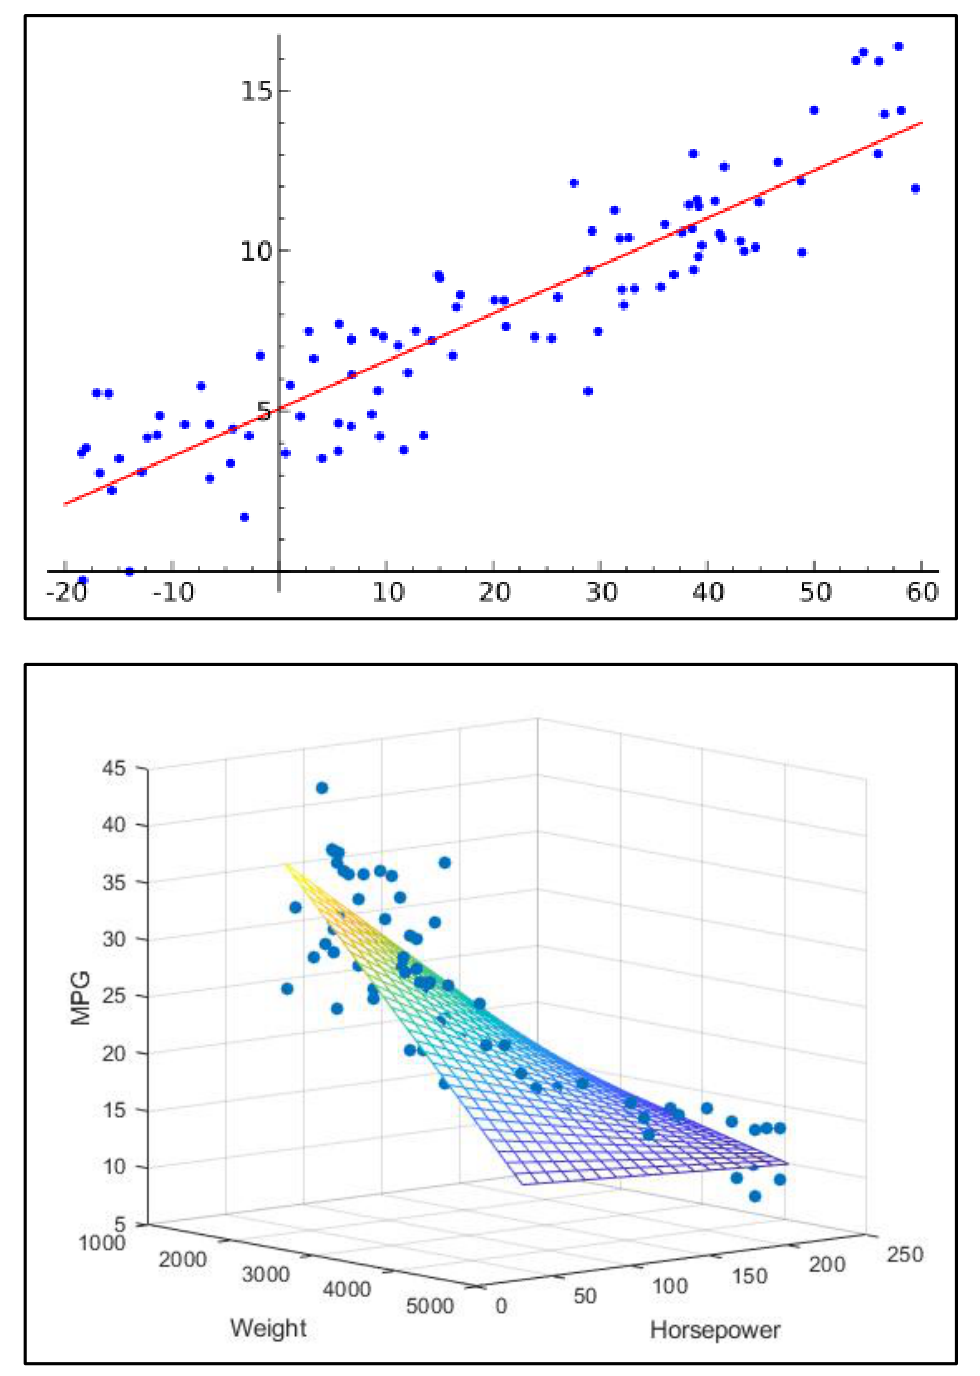
\includegraphics[width=\textwidth,height=3.8cm,keepaspectratio]{images/slide02_target_variables.png}
      \end{center}
    \end{column}
  \end{columns}
\end{frame}

% Slide 3: The Regression Problem
\begin{frame}{مسئله رگرسیون و مقایسه با طبقه‌بندی}{\lr{The Regression Problem vs. Classification}}
  \begin{itemize}
    \item \textbf{مثال‌ها} (\lr{Examples})
    \begin{columns}[T]
      \begin{column}{0.48\textwidth}
        \textbf{پیش‌بینی آب‌وهوا} (\lr{Weather})
        \begin{itemize}
          \item وابسته: سرعت باد یا دمای هوا.
          \item توصیفی: دما، رطوبت، تغییر فشار جو.
        \end{itemize}
      \end{column}
      \begin{column}{0.48\textwidth}
        \textbf{بازار مسکن} (\lr{House Market})
        \begin{itemize}
          \item وابسته: قیمت نهایی خانه.
          \item توصیفی: تعداد اتاق‌ها، فاصله تا حمل‌ونقل عمومی، مساحت حیاط.
        \end{itemize}
      \end{column}
    \end{columns}
    \vspace{0.25cm}
    \item \textbf{رگرسیون در مقایسه با طبقه‌بندی} (\lr{Regression vs. Classification})
    \begin{itemize}
      \item \textbf{طبقه‌بندی:} (\lr{Classification}) الگوریتم همه برچسب‌های ممکن را می‌شناسد (مانند بله/خیر، کم/متوسط/زیاد). تمام برچسب‌ها در داده‌های آموزش آمده‌اند و خروجی همیشه یکی از همین برچسب‌هاست.
      \item \textbf{رگرسیون} \lr{(Regression)}: الگوریتم مقادیری از داده‌ها را می‌شناسد (مانند $18^\circ\mathrm{C}$ و $21^\circ\mathrm{C}$). مقدار پیش‌بینی‌شده می‌تواند مقداری جدید خارج از داده‌های آموزشی باشد (مانند $20^\circ\mathrm{C}$).
    \end{itemize}
  \end{itemize}
\end{frame}

% Slide 4: Switching from Classification to Regression
\begin{frame}{گذار از طبقه‌بندی به رگرسیون}{\lr{Switching from Classification to Regression}}
  \begin{itemize}
    \setlength{\itemsep}{10pt}
    \item بسیاری از رویکردهای طبقه‌بندی را می‌توان (با اعمال اصلاحاتی) برای مسائل رگرسیون نیز به کار گرفت.
    \item در ادامه این فصل، هر یک از این رویکردها بررسی خواهند شد:
    \begin{itemize}
      \setlength{\itemsep}{8pt}
      \item \textbf{$k$ نزدیک‌ترین همسایه:} \lr{$k$-Nearest-Neighbors $\rightarrow$ $k$-NN Regression}
      \item \textbf{درخت‌های تصمیم:} \lr{Decision Trees $\rightarrow$ Regression / Model Trees}
      \item \textbf{شبکه‌های عصبی مصنوعی:} \lr{ANNs $\rightarrow$ ANNs for Regression}
    \end{itemize}
  \end{itemize}
\end{frame}

% Slide 5: Outline
\begin{frame}{سرفصل مطالب فصل رگرسیون}{\lr{Course Outline}}
  \begin{itemize}
    \setlength{\itemsep}{4pt}
    \item رگرسیون \lr{$k$-NN} برای رگرسیون (\lr{KNN for Regression})
    \item معیارهای ارزیابی رگرسیون (\lr{Evaluation Metrics})
    \item درخت‌های رگرسیون و درخت‌های مدل (\lr{Regression Trees, Model Trees})
    \item رگرسیون خطی، ریج و لاسو (\lr{Linear, Ridge / Lasso Regression})
    \item رگرسیون هم‌نوا یا ایزوتونیک (\lr{Isotonic Regression})
    \item رگرسیون چندجمله‌ای (\lr{Polynomial Regression})
    \item رگرسیون محلی (\lr{Local Regression})
    \item شبکه‌های عصبی برای رگرسیون (\lr{ANNs for Regression})
    \item موازنه بایاس و واریانس (\lr{The Bias/Variance Tradeoff})
  \end{itemize}
\end{frame}
